\xchapter{Proposed algorithms for DSMDStP}{}
\label{sec:algorithms}
\acresetall

In this chapter we describe an approximation algorithm and a heuristic for DSMDStP. 
%Throughout the description of the solutions, we give lemmas and theorems and as necessary we prove them. 
For the approximation algorithm, we give an upper bound for the maximum out-degree. As mentioned before, 
we were not able to guarantee the given spanning factor. For both solutions, we give an upper bound to the final costs of the arborescence's paths. 
For each solution, we give detailed information about the complexity. We also describe how the Multiple Set-Cover problem is solved, 
since it is an essential part of our algorithms. But the reader can skip this last section without impairing the reading.

\section{An Approximation Algorithm for DSMDStP}
\label{sec:algorithm}

Our algorithm is based on the algorithm presented in \cite{Elkin2006} (\emph{Directed Telephone Multicast Problem}). 
We modified it to address the spanner property. 

The algorithm has two phases. In the first phase the algorithm computes a so-called $\sqrt{l}$-partition. In this phase, some of the terminals are covered.
In the second phase, an instance of the Multiple Set-Cover problem (defined in \cite{Elkin2006}) is used to determine paths to cover the remaining terminals.

%In DTMP, the communication is assumed to happen in rounds and in each round every node is allowed to choose one of its neighbours and to send him a message. 
%The goal of DTMP is to find a schedule with the minimum number of rounds to deliver a message from a given node $s$ to a given set of nodes. 

\vspace{0.1cm}
\noindent \textbf{Preliminaries}
%\label{sec-topology-control}
\vspace{0.1cm}

The algorithm has a directed graph $G=(V, E)$ as input. The set $V$ is divided into two disjoint sets: $C$, the set of \emph{covered} nodes, and $U$, the set of \emph{uncovered} nodes. 
%Initially, $C$ contains only $s$. The other nodes of $V$ are in $U$. 
Let $UT = U \cap T$ (the set of uncovered terminals) and 
$CT = C \cap T$ (the set of covered terminals). 

Let $l = |T|$ and $d^*$ be the maximum out-degree of an optimum solution for an instance of DSMDStP ($d^* \leq l$). 
The \emph{out-neighbourhood} of $u$ in $G$ is denoted $N(u, G)$,
i.e. $N(u, G) = \{v : (u, v) \in E\}$. For a set of nodes $S$, $N(S, G)$ is the union of the sets $N(u, G), \forall u \in S$.

Let us denote $G(S)$ the graph induced by a set of nodes $S$. The graph induced by $U$ is thus denoted $G(U)$.
The $\Delta$-\emph{neighbourhood} of a node $u \in U$, denoted $\Delta$-neigh($u$), is the node set 
%$\{ t :$ $t \in T$ $\land$ $dist(s,u,G) + dist(u,t,G(U)) \leq k \cdot sp(s,t,G) \}$. 
\begin{center}
$\Delta$-neigh$(u) = \{ t :$ $t \in UT$ $\land$ $dist(s,u,G) + dist(u,t,G(U)) \leq k \cdot dist(s,t,G) \}$.
\end{center}

\begin{figure}[t]
\centering
\subfigure{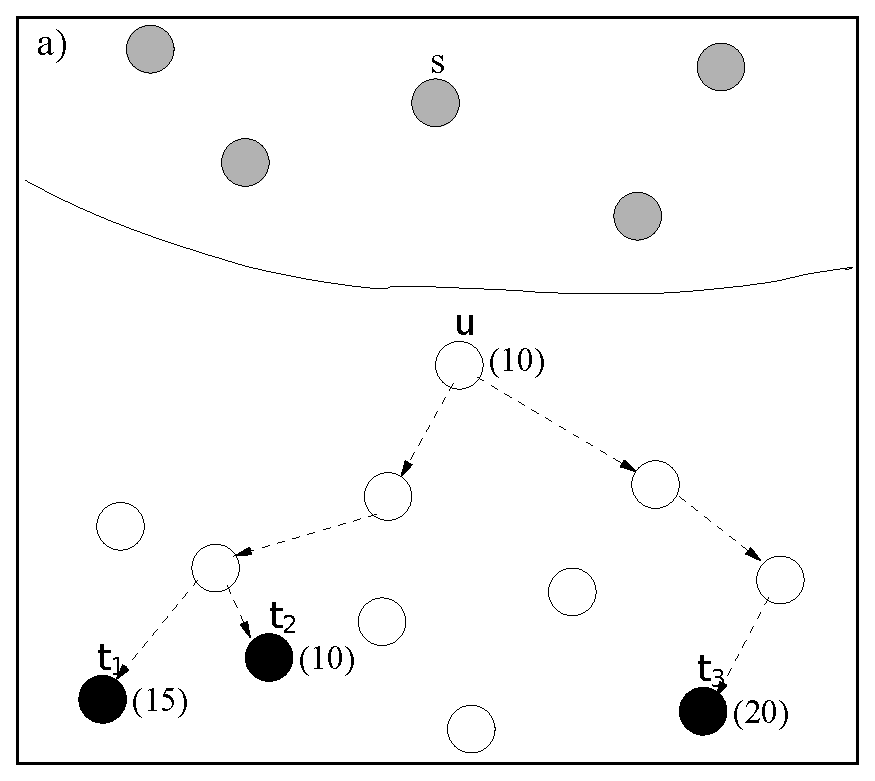
\includegraphics[scale=0.45]{imagens/neigh_teste}}
\subfigure{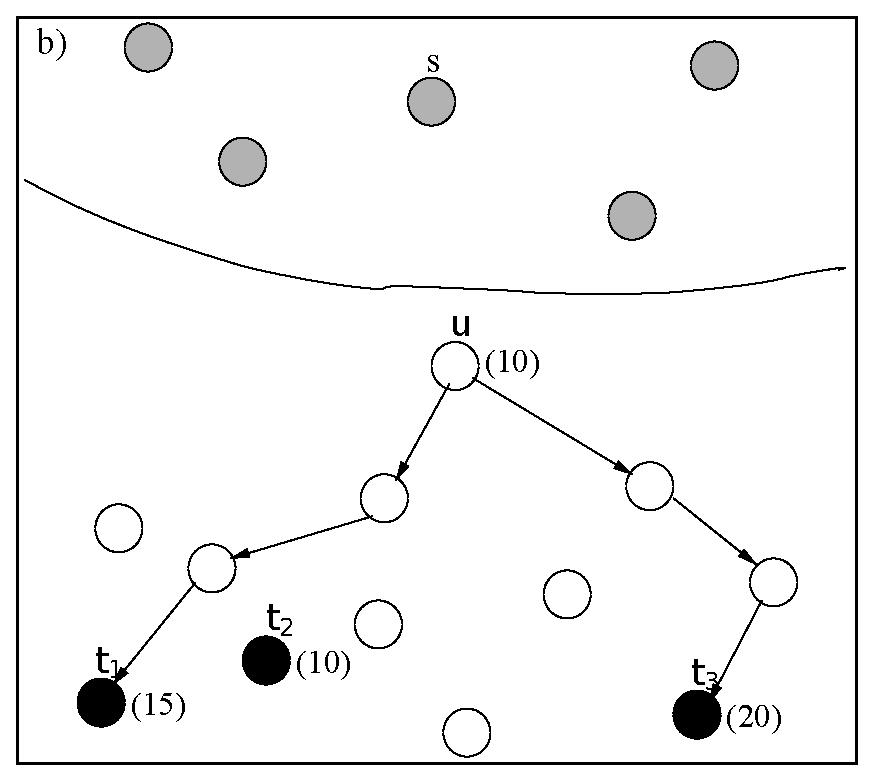
\includegraphics[scale=0.45]{imagens/neigh_color_teste}}
\caption[$\Delta$-neighbourhood of node $u$]{$\Delta$-neighbourhood of node $u$.
%Considering the quantity plotted in the right side of a node $v$ as equal to $dist(s,v,G)$ and considering $dist(u,t_1,G(U)) = 15$, $dist(u,t_2,G(U)) = 12$, $dist(u,t_3,G(U)) = 25$, 
%so $\Delta$-neigh$(u) = \{ t_1,t_3 \}$.
}
\label{fig:delta_neigh}
\end{figure}

Figure \ref{fig:delta_neigh} illustrates the concept of $\Delta$-neighbourhood. The gray nodes represent covered nodes (which are above the division) and the others are 
uncovered nodes (including the black ones which represent terminals in $UT$). Consider $k = 2$ and the quantity plotted in the right side of a node $v$ as equal to $dist(s,v,G)$ and consider 
$dist(u,t_1,G(U)) = 15$, $dist(u,t_2,G(U)) = 12$, $dist(u,t_3,G(U)) = 25$, The dashed paths in 
Figure \ref{fig:delta_neigh}a represent the shortest paths from $u$ to reachable terminals ($t_1$, $t_2$, $t_3$). In Figure \ref{fig:delta_neigh}b, the solid paths represent 
the paths to terminals only that are in $\Delta$-neigh$(u)$, which are $t_1$ and $t_3$.

%\begin{figure}[ht]
%\begin{minipage}[b]{0.46\linewidth}
%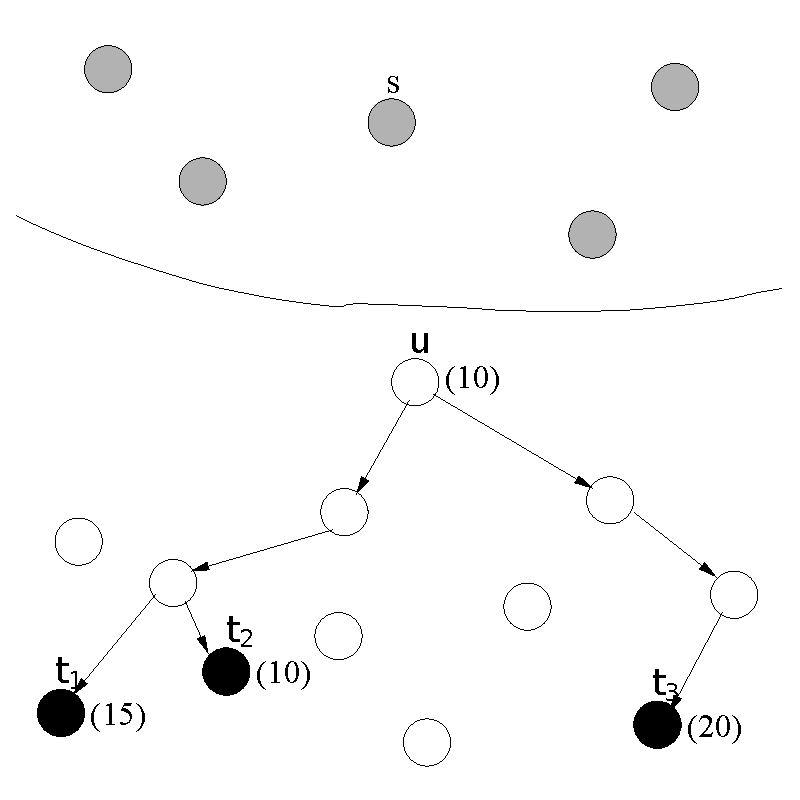
\includegraphics[scale=0.35]{imagens/neigh}
%\caption{PICS spanning factor}
%\label{fig:sigma_interference}
%\end{minipage}
%\hspace{0.3cm}
%\begin{minipage}[b]{0.46\linewidth}
%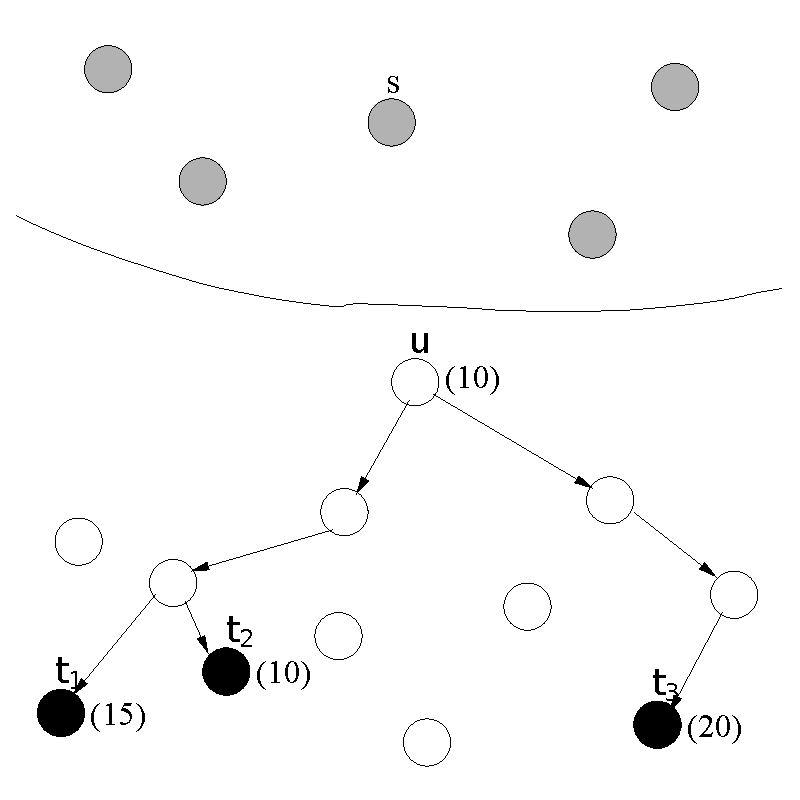
\includegraphics[scale=0.35]{imagens/neigh}
%\caption[]{Maximum PICS spanning factor}
%\label{fig:max_sigma_interference}
%\end{minipage}
%\end{figure}

We denote $SPT(s, S_{leaves}, G)$ a tree rooted at $s$ composed of shortest paths in graph $G$ from $s$ to each of the nodes in $S_{leaves}$.
Finally, for a graph $G$ or a path $P$ we denote $V(G)$ and $E(G)$ as well as $V(P)$ and $E(P)$ the sets of nodes and edges, respectively, of the graph and of
the path.

%informar como derivar o valor de d* (inclusive, isto eh um detalhe da implementaᅵᅵo).

%\subsection{General Description of the Algorithm}
%
%The algorithm has a directed graph $G=(V, E)$ as input and generates a graph $G_{out}=(V_{out}, E_{out})$ as output, which contains a multicast tree. 
%
% where, at the final of this procedure, 
%there is no $\sqrt{k}-bad$ vertex. 
%%Both definitions will be defined later but 
%The idea is to impose a bound on the maximum degree of the arborescences 
%that will be formed in the final of the second phase of the algorithm (whose nodes are uncovered) and at the same time impose a first bound on the degree of the 
%covered nodes at the final of first phase. After the first phase (i.e., after the computation of the $\sqrt k$ \emph{Partition}), there will be an arborescence 
%spanning $s$ and $CT$ with bounded degree. Let us call this arborescence $A_{\sqrt{k}-Par}$.
%%Since the arborescences that will be formed at the final of second phase are formed 

\subsection{First Phase: Computing a $\sqrt{l}$-Partition}

%A \mbox{$\sqrt k$-\emph{partition}}
%is a partition of the elements in $V$ in $m$ partitions $V_1, V_2, ..., V_m$ such that no partition has a \mbox{$\sqrt{k}$-bad} vertex. 
%A vertex $u$ is called a \mbox{$\sqrt{k}$-\emph{bad}} vertex in partition $V_i$ iff $u$ contains more than $\sqrt{k}$ 
%terminals in its $\Delta$-neighborhood. As no partition has a \mbox{$\sqrt{k}$-bad}

In the first phase, the algorithm computes a \mbox{$\sqrt{l}$-\emph{partition}}. 
A \emph{$\sqrt{l}$-partition} divides $V$ into the disjoint and non-empty sets $C$ and $U$, $V = C$ $\cup$ $U$, $C$ $\cap$ $U = \emptyset$, \linebreak
%$U \ne \emptyset$, 
$s \in C$, such that the $\Delta$-neighbourhood of any node in $U$ contains at most $\sqrt{l}$ terminals. A \mbox{$\sqrt{l}$-partition} is computed 
% me parece que esta condicao eh valida nao apenas para UT, mas tambem CT
by eliminating $\sqrt{l}$-\emph{bad} nodes. A node $u$ is called a \mbox{$\sqrt{l}$-\emph{bad}} node if $u$ contains more than $\sqrt{l}$ 
terminals in its \mbox{$\Delta$-neighbourhood}. Procedure \verb|CompPar| (from \cite{Elkin2006}) computes a $\sqrt{l}$-partition.

\begin{figure}[t]
\centering
\subfigure{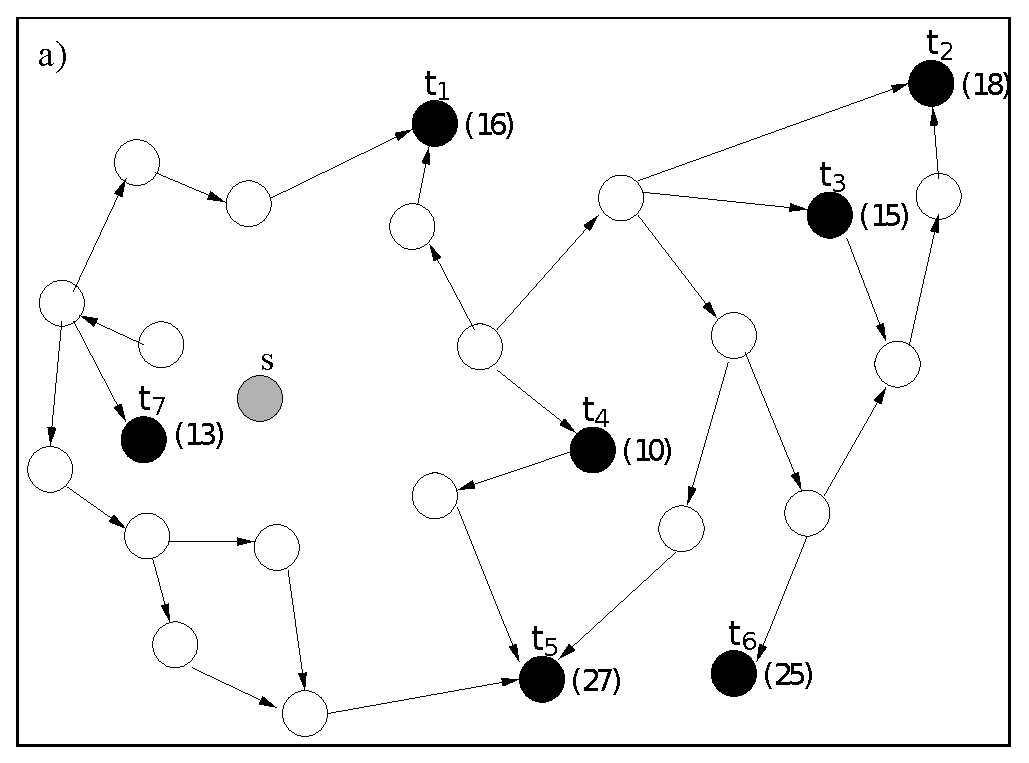
\includegraphics[scale=0.31]{imagens/compPar_teste}}\\
\subfigure{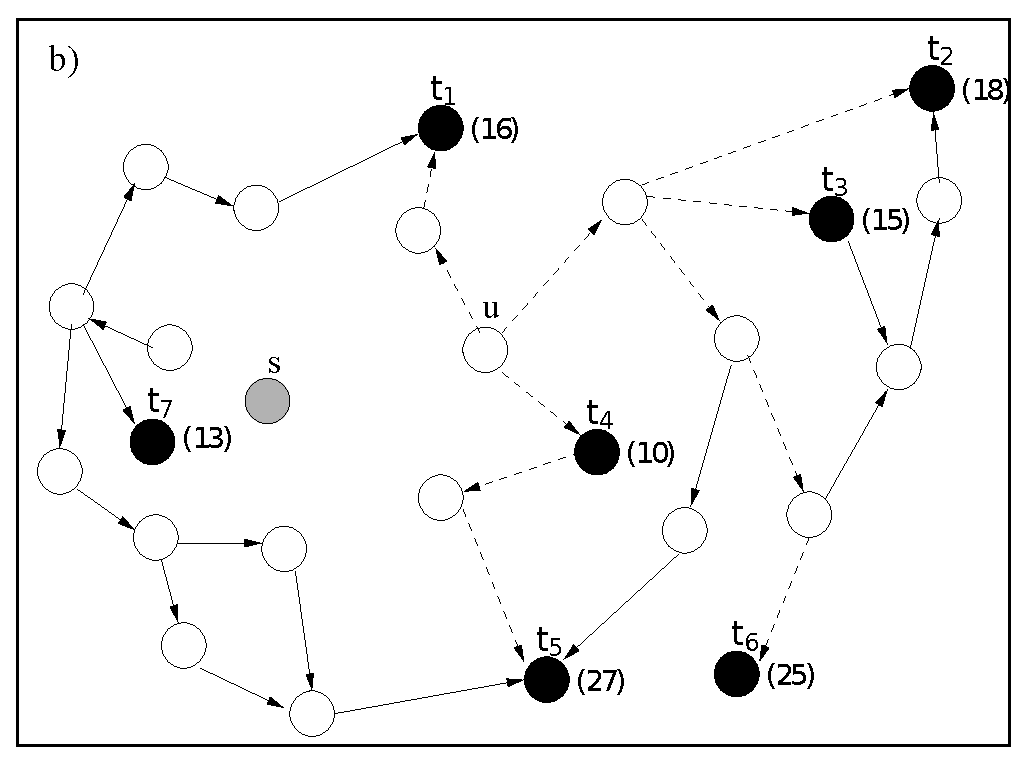
\includegraphics[scale=0.31]{imagens/compPar_bad1_teste}}
\subfigure{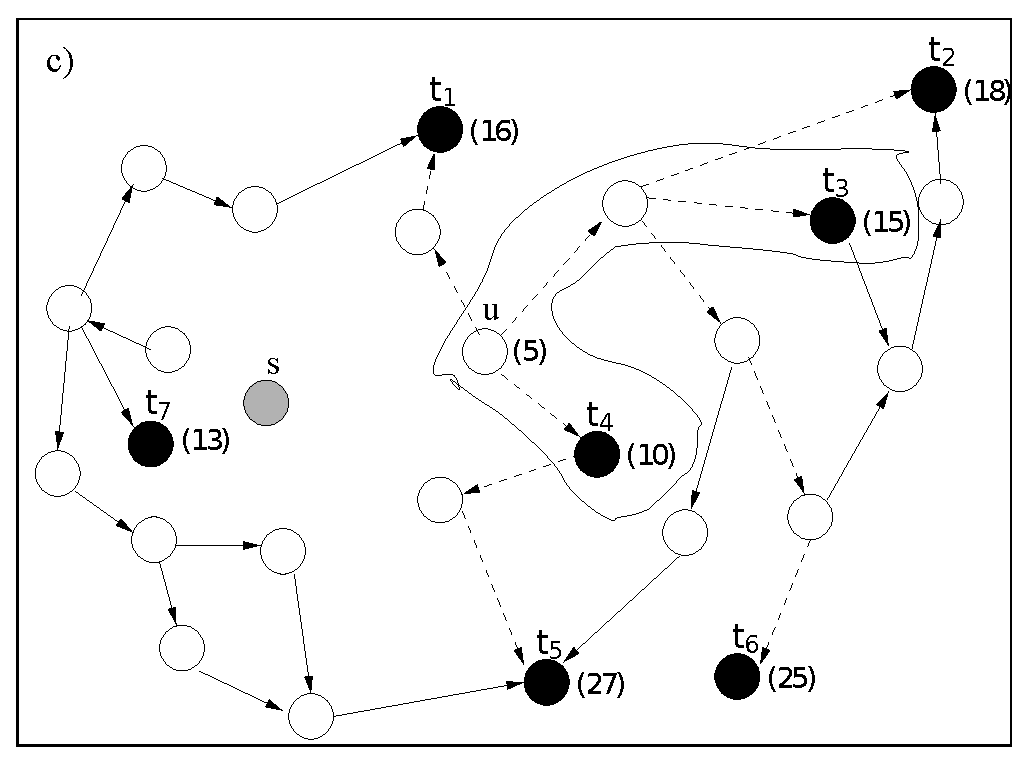
\includegraphics[scale=0.31]{imagens/compPar_tree1_teste}}
\subfigure{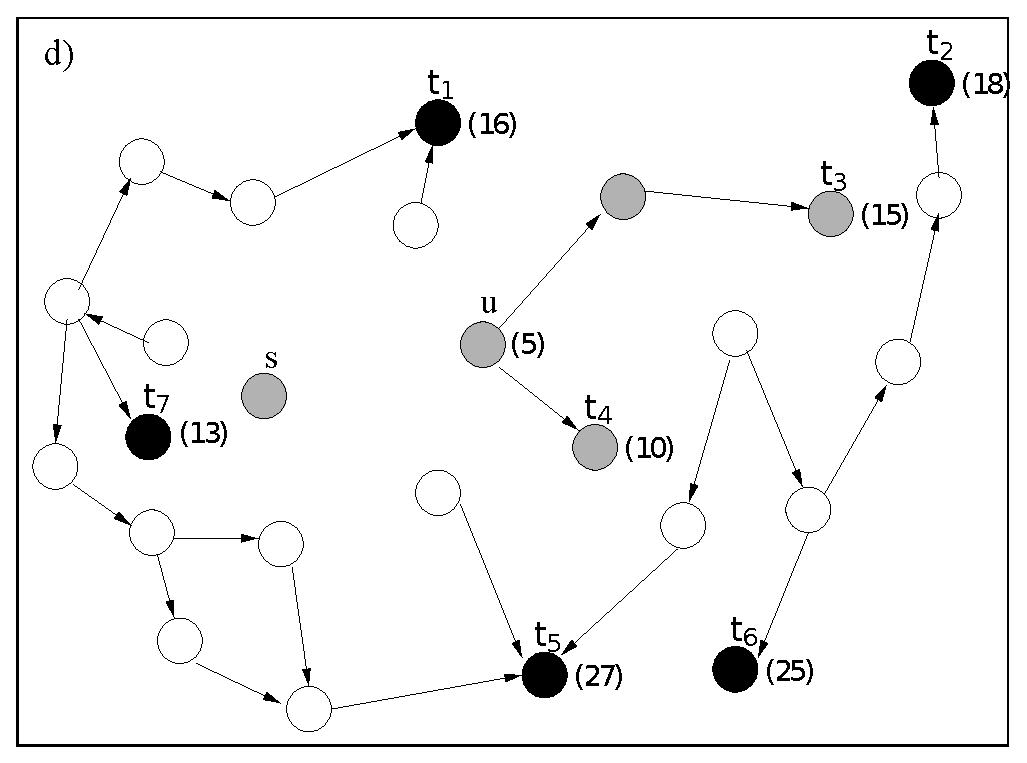
\includegraphics[scale=0.31]{imagens/compPar_cov1_teste}}\\
\subfigure{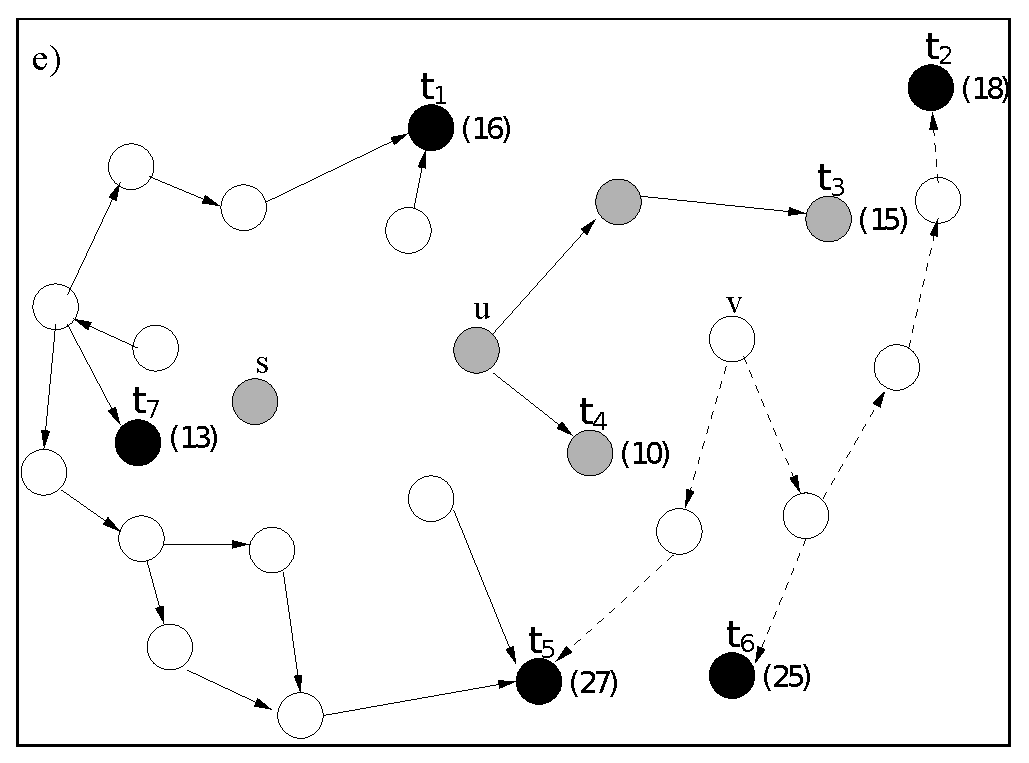
\includegraphics[scale=0.31]{imagens/compPar_bad2_teste}}
\subfigure{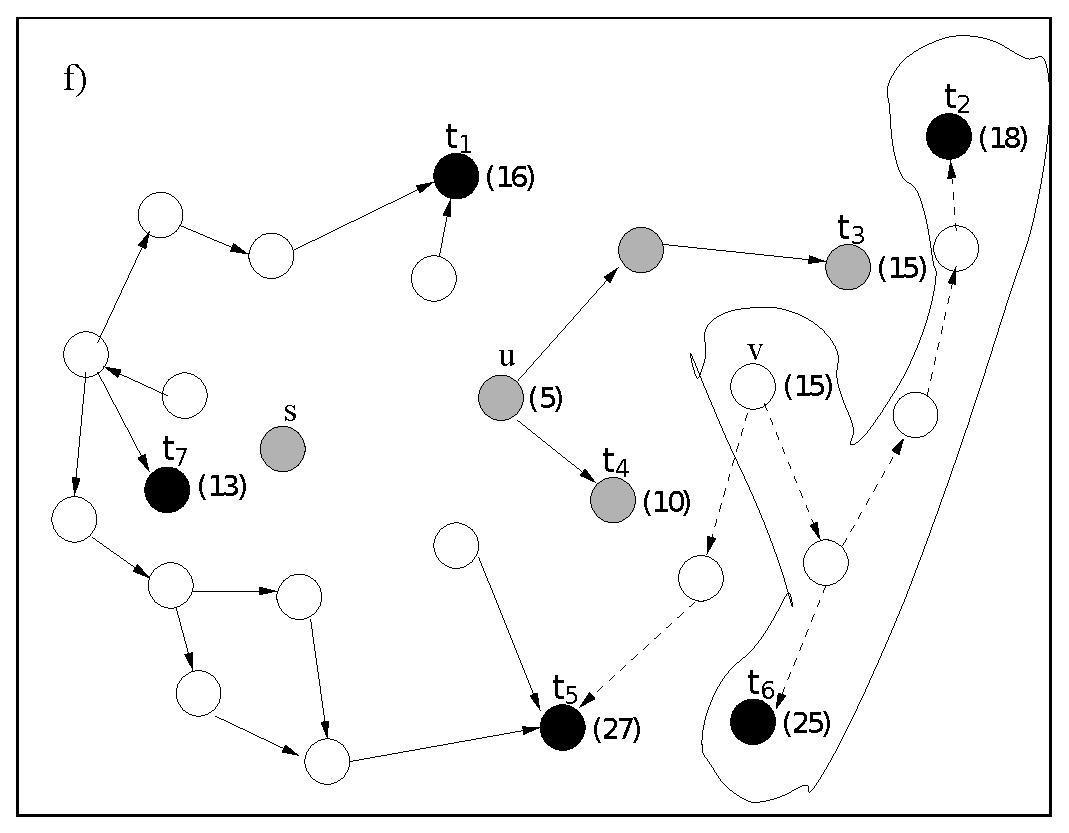
\includegraphics[scale=0.29]{imagens/compPar_tree2_teste}}
\subfigure{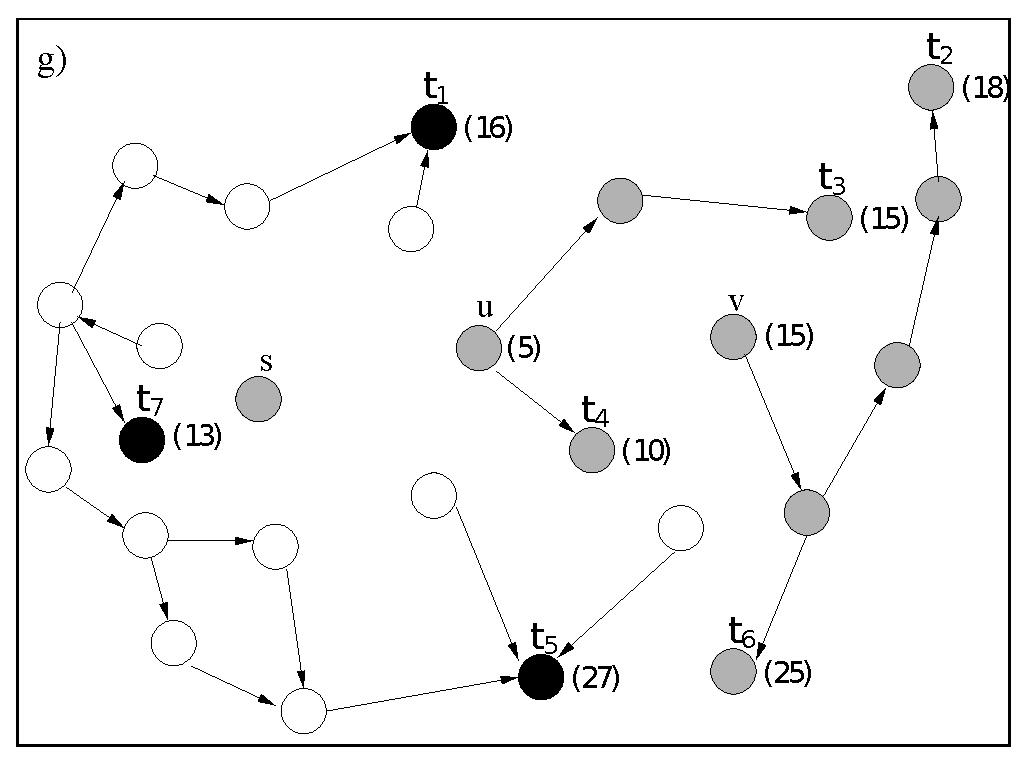
\includegraphics[scale=0.31]{imagens/compPar_cov2_teste}}
\caption[Applying procedure \emph{CompPar}]{Applying procedure \emph{CompPar}.} 
\label{fig:compPar}
\end{figure}

Figure \ref{fig:compPar} illustrates the application of procedure \verb|CompPar|. Gray nodes represent covered nodes and the others are uncovered nodes. 
Consider $k = 2$ and the quantity plotted in the right side of a node $z$ as equal to $dist(s,z,G)$ and consider 
$d(u,t_4,G(u)) = 5$, $d(u,t_3,G(u)) = 10$, $d(u,t_1,G(u)) = 11$, $d(u,t_2,G(u)) = 13$, $d(u,t_6,G(u)) = 20$, $d(u,t_5,G(u)) = 22$, 
$d(v,t_6,G(u)) = 10$, $d(v,t_2,G(u)) = 20$, $d(v,t_5,G(u)) = 24$. 
The dashed paths lead a $\sqrt{l}$-bad node $x$ to $\Delta$-neigh$(x)$ and the circled areas represent the trees removed 
from $G(U)$ and rooted at a previous $\sqrt{l}$-bad node. So, $Roots = \{ u,v \}$.



\begin{procedure}
\label{alg:compute_partition}
$C \gets \lbrace s \rbrace$, $U \gets V \setminus \lbrace s \rbrace$, $Roots \gets \emptyset$\\
\While{$G(U)$ contains a $\sqrt{l}$-bad node $v$}{
  Let $Cl(v)$ be the $\lfloor \sqrt{l} \rfloor$ uncovered terminals closest to $v$ in $G(U)$\\
  Let $T_v$ be a shortest path arborescence leading from $v$ to $Cl(v)$ in $G(U)$\\
  $C \gets C \cup V(T_v)$, $U \gets U \setminus V(T_v)$, $Roots \gets Roots \cup \lbrace v \rbrace$\\
}
Let $H(V_H,E_H)$ be the forest formed by the union of $T_v$, $\forall v \in Roots$\\
Output $(C,U,Roots, H)$
\caption{CompPar(G=(V, E), s, k)} 
\end{procedure}


% where, at the final of this procedure, 
%there is no $\sqrt{k}-bad$ vertex. 
%%Both definitions will be defined later but 
%The idea is to impose a bound on the maximum degree of the arborescences 
%that will be formed in the final of the second phase of the algorithm (whose nodes are uncovered) and at the same time impose a first bound on the degree of the 
%covered nodes at the final of first phase. 

The following lemmas state that \verb|CompPar| computes a correct  
\mbox{$\sqrt{l}$-partition} and that the set $Roots$ has cardinality at most $\sqrt{l} + 2$ (these lemmas are
similar to Claims 2.2 and 2.3 in \cite{Elkin2006} and have analogous proofs - proofs are thus omitted). 
Lemma \ref{lem:proc_comppar} follows from the condition of stopping of the loop of \verb|CompPar| (line 2). 
Lemma \ref{lem:roots_cardinality} follows from the number of terminals removed in each iteration (line 3 of \verb|CompPar|) along with the number of terminals left to be removed in 
the last iteration.

\begin{Lem} 
\label{lem:proc_comppar}
\cite{Elkin2006} The pair $(C, U)$ output by procedure \verb|CompPar| is a \mbox{$\sqrt l$-\emph{partition}}. 
\end{Lem}

\begin{Lem} 
\label{lem:roots_cardinality}
\cite{Elkin2006} $|Roots| \le \sqrt{l} + 2$.
%nao estou convencido deste valor
\end{Lem}

After the computation of a $\sqrt{l}$-partition, we build a directed graph that contains a path from $s$ to each node $t$ in $CT$ that satisfies $k \cdot dist(s,t,G)$ and
which has bounded degree. Let us call this graph $G_{\sqrt{l}-Par}$. It is built as the union of a shortest path from $s$ to each node in $Roots$ and
the $T_v$ trees calculated in line 4 of \verb|CompPar| (represented by forest $H=(V_H, E_H)$, output by \verb|CompPar|). 
This is represented by procedure \verb|CompGraphFirstPh|. %\emph{\ref{alg:compute_arborescence}}.

\begin{procedure}
%$Roots \gets \ref{alg:compute_partition}$\\
$A_{Roots} \gets SPT(s,Roots,G)$\\
%$H(V_H,E_H) \gets \varnothing$\\
%\ForEach{$u \in Roots$}{
%  $H \gets H \cup T_u$\\
%}
%Let $S_{leaves}$ be the set of leaves of all $T_u$, $\forall u \in Roots$\\
$G_{\sqrt{l}-Par} \gets A_{Roots} \cup H(V_H, E_H)$\\
$C \gets V(G_{\sqrt{l}-Par})$, $U \gets V \setminus C$\\
Output $(C,U,G_{\sqrt{l}-Par})$
\caption{CompGraphFirstPh(G, s, Roots, H)} 
\label{alg:compute_arborescence}
\end{procedure}

%Since the arborescences that will be formed at the final of second phase are formed 

%  $A_{\sqrt{k}-Par}$ is computed as follows: compute the shortest path arborescence in $G$ from $s$ to the set $Roots$. Let this arborescence be $A_{roots}$. 
%$A_{\sqrt{k}-Par}$ is formed by the concatenation of $A_{roots}$ to $T_u$, for each $u \in Roots$.

\SetKwInOut{Input}{Input}
\SetKwInOut{Output}{Output}


\begin{Lem}
  \label{lem:roots_size}
%The maximum out-degree of nodes in $G_{\sqrt{k}-Par}$, $D_{max}(G_{\sqrt{k}-Par}), is \linebreak 
The maximum out-degree of nodes in $G_{\sqrt{l}-Par}$ is $\leq 2\sqrt{l} + 2$
%  \begin{proof}
%    $\forall v \in Roots$, $D_{max}(T_v) \leq \sqrt{k}$ (line 5 of \ref{alg:compute_partition}). Let the node $x$ of $H(V_H,E_H)$ be the node with  
%maximum degree and assume its degree as $\sqrt{k}$. When we apply SPT in line 4 of \ref{alg:compute_arborescence}, assume that $y \in V(A_{\sqrt{k}-Par})$ 
%is in the path for $u \in Roots$. If $y = x$ then $y$ is one of the roots in $Roots$ and the proof follows. Otherwise, 
%  \end{proof}
\end{Lem}
\begin{Proof}
The $T_v$ trees computed in line 4 of \verb|CompPar| are disjoint. Each node in these trees has degree at most $\sqrt{l}$,
as each $T_v$ is a shortest path tree to at most $\sqrt{l}$ terminals. $A_{Roots}$ is a shortest path tree from $s$ to the nodes in $Roots$. 
As the cardinality of $Roots$ is at most $\sqrt{l} + 2$ (Lemma \ref{lem:roots_cardinality}), each node in $A_{Roots}$
has degree at most $\sqrt{l} + 2$. As $G_{\sqrt{l}-Par}$ is the union of all these trees, the degree of any of its nodes is limited to $\sqrt{l} + \sqrt{l} + 2 = 2\sqrt{l} + 2$.
\end{Proof}

%\vspace{0.5cm}
%\noindent \textbf{Reducing the problem of cover \emph{UT} to the \emph{Multiple Set-Cover} problem}
%\vspace{0.5cm}

\subsection{Multiple Set-Cover Problem}
\label{sec:msc_definition}

As mentioned before, the MSC problem was stated in \cite{Elkin2003,Elkin2006}. A solution was proposed in \cite{Chekuri2004} based on an approximation algorithm 
for another problem, called \emph{Maximum Coverage with Group Budgets} (MCG). 
%The MSC is a minimization version of an optimization problem where the relative MCG problem consists in a maximization version.

Let $\beta(V_1,V_2,E)$ be a bipartite graph.  A set $S \subseteq V_1$ is called a \emph{set-cover} of $V_2$ if $N(S,\beta) = V_2$. 
The Multiple Set-Cover problem is stated as follows \cite{Elkin2006}:

\vspace{0.3cm}
\noindent \emph{Input}: A bipartite graph $\beta(V_1,V_2,E)$ with \mbox{$|V_1| + |V_2| = n$}. The set $V_1$ is partitioned into a disjoint union of sets 
\mbox{$V_1 = \bigcup_{j=1}^{d}A_j$}. 

\vspace{0.3cm}
\noindent \emph{Output}: A set-cover $S \subset V_1$ of $V_2$ which minimizes $val(S)$, where
\mbox{$val(S) = max\lbrace |S \cap A_i| \rbrace_{i=1}^{d}$}. Figure \ref{fig:msc} illustrates an example.
%\vspace{0.3cm}

\begin{figure}[t]
\centering
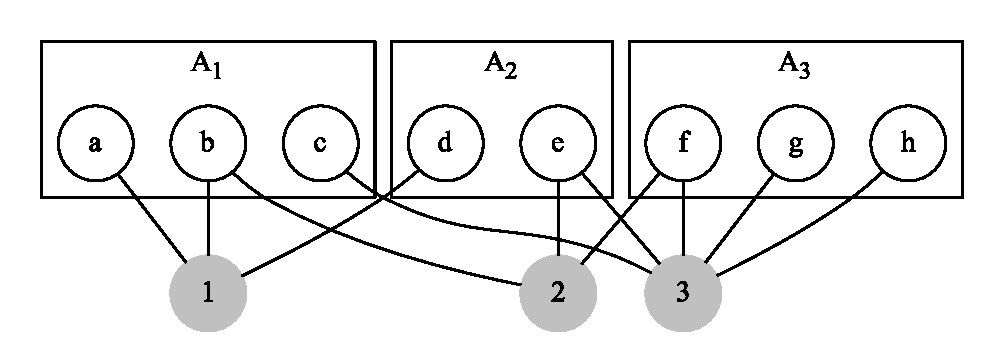
\includegraphics[scale=0.75]{imagens/msc_label}
\caption[Example of MSC]{Example of MSC. Consider $V_1 = \lbrace a,b,c,d,e,f,g,h \rbrace$, $V_2 = \lbrace 1,2,3 \rbrace$ and $A_1$, $A_2$, $A_3$ represent the partitions of $V_1$ ($V_1$ = $A_1 \cup A_2 \cup A_3$). 
The set-covers $S_1 = \lbrace a,e \rbrace$, $S_2 = \lbrace c,d,f \rbrace$ and $S_3 = \lbrace b,f \rbrace$ are examples of optimum solutions, since 
$val(S_1) = val(S_2) = val(S_3) = 1$.}
\label{fig:msc}
\end{figure}

\begin{Theo}
  \label{teorema:fator_aproximacao}
  \cite{Chekuri2004}. The multiple set-cover problem admits a polynomial time greedy $(\log |V_2| + 1)$-approximation algorithm.
\end{Theo}

  In section \ref{sec:solve_msc} we explain how MSC is solved.

\subsection{Second Phase: Covering Nodes in \emph{UT} using an Instance of the \emph{Multiple Set-Cover} Problem}
\label{sec:second-phase}

In the second phase, the remaining nodes in $UT$ become covered. As in \cite{Elkin2006}, we use an instance of the MSC problem
to find paths to cover these nodes while limiting the maximum node degree. 

The second phase is divided into two parts. First,
an instance of MSC is solved to find a specific subset of the covered nodes. In the second
part, we define paths from these covered nodes to the uncovered terminals. 
The union of these paths with $G_{\sqrt{l}-Par}$ generates a graph which contains an arborescence that is a solution
to DSMDStP. 

%Observes that in the construction 
%of $F$ we are concerned with only the degree of the roots of $F$. As we will argue better later, due to the way we define the paths to be considered 
%in the MSC instance and since we have eliminated $\sqrt{k}$-bad nodes (limiting the number of terminals in $UT$ reached through an uncovered node) 
%in the first phase, we only need to care about with the degree of the roots of $F$ that we call \emph{link} nodes (since they are linking covered nodes to 
%uncovered nodes).

The instance of MSC, $\beta=(V_1, V_2, \varepsilon)$, is defined as follows. $V_1$ is composed of \emph{pseudo nodes}. A pseudo node $x_{u, v}$ is created
for each edge $(u, v)$ such that $u$ is a covered node and $v$ is an uncovered node. Formally:
%\begin{displaymath}\label{v1}
\begin{center}
$V_1 = \lbrace x_{u,v} : u \in C, v \in U, (u,v) \in E \rbrace$.
\end{center}
%\end{displaymath}

The set $V_2$ is the set of uncovered terminals, i.e. \mbox{$V_2 = UT$}. The edge set $\varepsilon$ is defined as follows. There is an edge from
pseudo node $x_{u,v}$ to $t \in V_2$ iff the cost of a shortest path from $s$ to $u$ in $G$, plus the cost of $(u, v)$, plus the cost of a shortest path from
$v$ to $t$ in $G(U)$ satisfies the spanner property for $t$. I.e.: 

%\begin{equation}\label{eq:bipartite_edge}
%dist(u,v,G) + dist(v,t,G(U)) \leq \Delta_t.
%\end{equation}
\begin{center}
%\begin{displaymath}\label{eq:bipartite_edge}
$dist(s, u, G) + C(u, v) + dist(v,t,G(U)) \leq k \cdot dist(s,t,G)$.
\end{center}
%\end{displaymath}


Let $A_u = \lbrace x_{u,v} :  v \in N(u, G(U)) \rbrace$. The disjoint partition of $V_1$ that is input for the instance of the MSC problem is 
$V_1 = \bigcup_{u \in C}A_u$. Each partition $A_u$ represents the set of uncovered neighbours of node $u$ in $G(U)$. As there is an algorithm
to MSC that limits \mbox{$A_u$ $\cap$ $S$}, MSC is used to provide a bound to node degree in the final arborescence.

\begin{figure}[t]
\centering
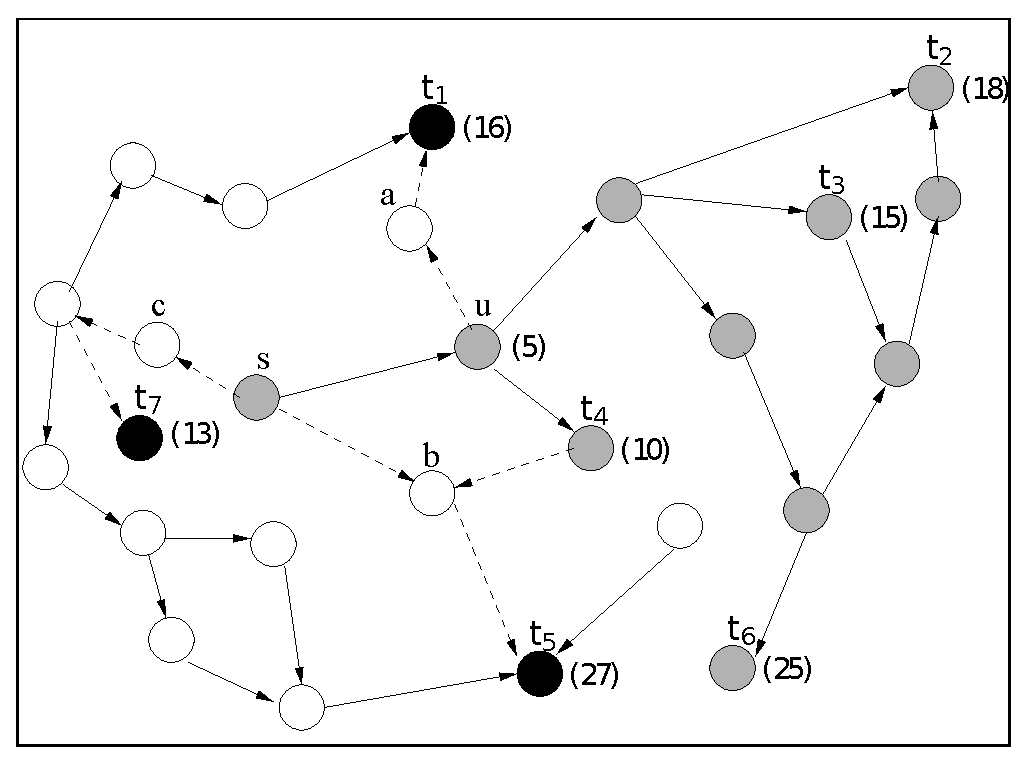
\includegraphics[scale=0.45]{imagens/mscInstance_teste}
\caption[Setting an MSC instance]{Setting an MSC instance.}
\label{fig:mscInstance}
\end{figure}

Figure \ref{fig:mscInstance} illustrates how an MSC instance is set. Gray nodes represent covered nodes and the others are uncovered nodes. 
A dashed path lead a covered node $x$, followed by an uncovered node $y$, to a terminal $t \in UT$ s.t. $dist(s,x,G) + C(x,y) + dist(y,t,G(U)) \le k \cot dist(s,t,G)$. 
We can set $\beta=(V_1, V_2, \varepsilon)$ as $V_1 = \{ X_{u,a}, X_{t_4,b}, X_{s,b}, X_{s,c} \}$, where the disjoint partition of $V_1$ can be represented by the set $\{ \{ X_{u,a} \}, \{ X_{t_4,b} \}, \{ X_{s,b}, X_{s,c} \} \}$, 
$V_2 = \{ t_1, t_5, t_7 \}$, and $\varepsilon = \{ (X_{u,a}, t_1), (X_{t_4,b}, t_5), (X_{s,b}, t_5), (X_{s,c}, t_7) \}$.

%In the optimum DCCMDSttT, $d^* \geq 2$, since the optimum Steiner tree could be a binary tree. We may assume that $d^* \leq k$.

%lemmas

The following lemmas present properties of solutions for such an MSC instance. Their proofs are similar to the 
proofs of Lemmas 3.3 and 3.4 in \cite{Elkin2006}. So we only provide the main idea of the proofs.

\begin{Lem}
  \label{lem:val_solution}
  A  multiple set-cover instance $\beta=(V_1, V_2, \varepsilon)$, as defined above, admits a solution $S^* \subseteq V_1$ such that $val(S^*) \leq d^*$.
\end{Lem}
\begin{Proof}
Let $T^*$ be an optimal solution to an instance of DSMDStP. For any node $t \in UT$, there is a path from $s$ to $t$ in $T^*$. Let $u$ be the last node of this
path that is in $C$ and $v$ the node after $u$ on this path ($v \in U$). So there will be a pseudo node $x_{u, v}$ in $V_1$ and an edge $(x_{u, v}, t) \in \varepsilon$.
As this happens to all nodes in $UT$ and $T^*$ has maximum degree $d^*$, there is a solution $S^*$ for $\beta$ such that
%each pseudo node $x_{u, v}$ will cover at most $d^*$ terminals in $V_2$, as $x_{u, v} \in S^*$ iff $v$ is a child of $u$ in $T^*$. Thus,
for each node $u$ there will be at most $d^*$ pseudo nodes $x_{u,v}$ in the solution $S^*$, as $x_{u, v} \in S^*$ iff $v$ is a child of $u$ in $T^*$. Thus,  
$max_{c \in C}\{|S^* \cap A_c|\}\le d^*$.
\end{Proof}

\begin{Lem}
  \label{lem:max_pseudo_node_degree}
 Let $D$ be a solution to $\beta=(V_1, V_2, \varepsilon)$ with partition $V_1 = \bigcup_{v \in C}A_v$ using Algorithm \ref{alg:greedy} (presented in \cite{Chekuri2004}). 
Then $max_{v \in C}|D \cap A_v| = (\log{l}+1)\cdot d^*$.
\end{Lem}
\begin{Proof}
As $d^*$ is greater than or equal to $val(S^*)$ for an optimal solution $S^*$ of $\beta$ and $|V_2| \le l$, this lemma is a direct application of Theorem \ref{teorema:fator_aproximacao}.
\end{Proof}

In order to build the final solution to DSMDStP, we first add to $G_{\sqrt{l}-Par}$ a set of shortest 
paths from covered nodes to terminals in $UT$ and compute a shortest path arborescence over the resulting graph.
We use $D$ to choose the covered nodes. The complete algorithm to DSMDStP is given in the section \ref{sec:complete_algorithm}. 

\subsection{The Complete Algorithm}
\label{sec:complete_algorithm}

Algorithm \ref{alg:approximation} represents the complete algorithm. Lines 1-2 represent the first phase.
After computing a $\sqrt{l}$-partition (line 1), graph $G_{\sqrt{l}-Par}$ is computed (line 2).
%Lines 4-13 correspond to the second phase of the algorithm. In lines 4-5 represent the instance of the MSC problem (first part of the second phase).
Lines 3-4 correspond to the first part of the second phase of the algorithm, i.e. the application of the algorithm in \cite{Chekuri2004} to an instance of the MSC problem
(as described in Section \ref{sec:second-phase}). 
The output of this algorithm is the set $D$, whose elements cover $V_2$. 
Lines 5-12 correspond to the second part of the second phase, when the arborescence that is output of the algorithm is built.

In lines 5-10 the digraph $\varGamma(V_{\varGamma},E_{\varGamma})$ is built. For each uncovered node $t$ in $UT$, we choose a node $x_{u, v}$ in $D$
such that there is an edge $(x_{u, v}, t) \in \varepsilon$ and $C(u, v) + dist(v,t,G(U))$ is minimum. The set $V_\varGamma$ is composed of the nodes $u$ and the set of nodes on a shortest path
from $v$ to $t$. The set $E_\varGamma$ contains the edges in these paths and edges $(u, v)$.

In line 11, we build the graph $G_f$, which is the union of graphs $G_{\sqrt{l}-Par}$ and $\varGamma$. 
We finally compute the arborescence $\mathcal{A}_f$ that is the output of the algorithm. $\mathcal{A}_f$ is a shortest
path tree in $G_f$ rooted at $s$, containing shortest paths from $s$ to the terminals. 

\SetKwInOut{Input}{Input}
\SetKwInOut{Output}{Output}
%\SetKwComment{coment}{\{}{\}}

\begin{algorithm}
\Input{$G=(V, E)$, $s \in V$, $T \subset V$, $k$}
\Output{$\mathcal{A}_f =(V_{\mathcal{A}_f}, E_{\mathcal{A}_f})$}
\BlankLine
  %$C \gets s$, $U \gets V \setminus \lbrace s \rbrace$\\
  $(C, U, Roots, H) \gets$ \verb|CompPar|($G, s, k$) \\ %\coment{Run Procedure \emph{\ref{alg:compute_partition}} to compute the $\sqrt{k}$ Partition}
  $(C, U, G_{\sqrt{l}-Par})\gets\verb|CompGraphFirstPh|(G,s,Roots,H)$ \\	
  Build the MSC instance $\beta = (V_1, V_2, \varepsilon)$ as in Section \ref{sec:second-phase} \\
  $D \gets $ Apply approximation algorithm \cite{Chekuri2004} on $\beta$\\
  $\varGamma(V_{\varGamma},E_{\varGamma}), V_{\varGamma} \gets \emptyset, E_{\varGamma} \gets \emptyset$\\
%  \ForEach{$x_{u,v} \in D$}{
%    $S_{ter} \gets \lbrace t : t \in V_2 \wedge (x_{u,v},t) \in \varepsilon \rbrace$ \\
%    \ForEach{$t \in S_{ter}$}{
%           $s \gets sp(u,t,G(U))$ \\
%           $V_{\varGamma} \gets V_{\varGamma} \cup V(s)$ \\ 
%    	  $E_{\varGamma} \gets E_{\varGamma} \cup E(s)$ \\
%	}
%  }
  \ForEach{$t \in V_2$}{
    Choose $x_{u, v} \in D$ : $(x_{u, v}, t) \in \varepsilon$ and $C(u, v) + dist(v,t,G(U))$ is minimum \\
    $s \gets sp(v, t, G(U))$ \\
    $V_{\varGamma} \gets V_{\varGamma} \cup \{u\} \cup V(s)$ \\ %, \forall q, q \in S_{ter}$\\% \wedge q \notin V_{\varGamma}$ \\
    $E_{\varGamma} \gets E_{\varGamma} \cup \{(u, v)\} \cup E(s)$ \\ %, \forall q, q \in S_{ter}$\\% \wedge q \notin V_{\varGamma}$ \\

 }
  $G_f \gets G_{\sqrt{l}-Par} \cup \varGamma(V_\varGamma,E_\varGamma)$ \\
  $\mathcal{A}_f \gets SPT(s, T, G_f)$

%  $\forall x_{u,v} \in D$, add $u$ to $S_{PS}$\\
%  %PS - possible sources
%  $F(V_F,E_F) \gets$ Apply Prim's algorithm to $\varGamma(V_{\varGamma},E_{\varGamma})$ considering the sources $S_{PS}$ and destinations $UT$\\
%  $A_{final} \gets A_{\sqrt{k}-Par} \cup F(V_F,E_F)$

\caption{Approximation Algorithm to \mbox{DSMDStP}} 
\label{alg:approximation}
\end{algorithm}


\begin{Lem}
  \label{lem:max_degree}
  The maximum out-degree of nodes in $G_f$ is $\leq 2\sqrt{l} + 2 + O(\log l) \cdot d^*$.
\end{Lem}
  \begin{Proof}
The algorithm adds nodes to $G_f$ in the first and second phases of the algorithm. After the first phase, each node in $G_f$ has
maximum out-degree $2\sqrt{l} + 2$ (Lemma \ref{lem:roots_size}). In the second phase, new nodes are added to $G_f$ and the out-degree of
nodes already in $G_f$ might increase. The new added nodes have maximum degree $\sqrt{l}$, as, in this phase, there are no more $\sqrt{l}$-bad
nodes. The nodes already in $G_f$ that might have their degrees increased are those nodes $u$ for which there is a pseudo node $x_{u, v}$ in $D$. 
However, from Lemma \ref{lem:max_pseudo_node_degree}, the out-degree of these nodes might be increased by at most $O(\log l) \cdot d^*$. 
Thus, the maximum out-degree of any node is $2\sqrt{l} + 2 + O(\log l) \cdot d^*$.
  \end{Proof}

\begin{Lem}
  \label{lem:cost_guaranteed}
$\forall t \in T$, $dist(s,t,G_f) \leq k \cdot ( dist(s,t,G) + dist(s,t_{max},G))$, 
where $t_{max} \in \{t' | 
(t' \in T) \land (\forall t'' \in T : dist(s,t'',G) \le dist(s,t',G))\}$.
\end{Lem}
  \begin{Proof}
If $t$ is covered in the first phase, 
$dist(s, t, G_f) \le k \cdot dist(s,t,G)$ by construction: a tree rooted at a (previously) $\sqrt{l}$-bad node $u$ contains paths from $u$ to terminals $t$ such that 
$dist(s, u, G) + dist(u, t, G) \le k \cdot dist(s,t,G)$. In particular, all nodes $v$ (terminals or not) that are covered in the first phase, are in a path
from $s$ to a terminal $t$ with cost less than or equal to $k \cdot dist(s,t,G)$, which is $\le k \cdot dist(s,t_{max},G)$. 

For the terminals $t$ that are only covered in the second phase (as in the proof of Lemma \ref{lem:val_solution}, for each $t$, there is 
a path between $s$ and $t$), observe that
a pseudo node $x_{u, v}$ and an edge $(x_{u, v}, t)$ are inserted in the input graph to the MSC instance 
if $dist(s, u, G)+C(u,v)+dist(v,t,G(U)) \leq k \cdot dist(s,t,G)$. Thus, in particular, $C(u,v)+dist(v,t,G(U)) \le k \cdot dist(s,t,G)$.
As $dist(s, u, G) \le k \cdot dist(s,t_{max},G)$, we have
$dist(s,t,G_f) \leq k \cdot (dist(s,t,G) + \cdot dist(s,t_{max},G))$.
  \end{Proof}

By Lemma \ref{lem:cost_guaranteed}, the algorithm can violate the spanner property for some terminals. Observe, however, that this might only happen
to terminals covered in the second phase. Terminals covered in the first phase have their spanner constraint satisfied.

\begin{Theo}
  \label{teorema:final_theorem}
  The approximation algorithm generates an arborescence $\mathcal{A}_f$ with bounded out-degree $2\sqrt{k} + 2 + O(\log l) \cdot d^*$ and that 
has paths from $s$ to each terminal $t \in T$ with cost less than or equal to $k \cdot ( dist(s,t,G) + dist(s,t_{max},G))$, 
where $t_{max} \in \{t' | 
(t' \in T) \land (\forall t'' \in T : dist(s,t'',G) \le dist(s,t',G))\}$.
\end{Theo}
  \begin{Proof}
The $\mathcal{A}_f$ tree is generated by computing minimum cost paths in $G_f$ from $s$ to each $t \in T$. The theorem follows from the fact that
all nodes in $G_f$ have out-degree $\le 2\sqrt{l} + 2 + O(\log l) \cdot d^*$ (Lemma \ref{lem:max_degree}) and that $G_f$ contains paths from $s$ to each $t \in T$ 
with costs $\le k \cdot ( dist(s,t,G) + dist(s,t_{max},G))$ (Lemma \ref{lem:cost_guaranteed}).
  \end{Proof}

%In order to evaluate the bound on node-degree of the algorithm, it was proved that there is no sublogarithmic approximation to the 
%Steiner version of the \emph{Minimum Degree Spanning Tree} (MDS) in digraphs \cite{Fraigniaud2001}, which is a restriction of DSMDStP.

\subsection{Complexity}

The \verb|CompPar| procedure has its complexity bounded by $(\sqrt{|T|} + 2)O(|V|^3)$ due to the number of loop iterations (Lemma \ref{lem:roots_cardinality}) and 
the complexity of building a shortest path tree (SPT) for the $\sqrt{l}$-bad node candidates, using Dijkstra's algorithm \cite{Cormen2009}. The complexity of the procedure \verb|CompGraphFirstPh| 
is bounded by the running time of building SPT, so it is bounded by $O(|V|^2)$.

The complexity of building the MSC instance (line 3) is related to the complexity of composing the sets $V_1$ and $\varepsilon$. 
The former is bounded by $O(|V|^2)$ 
where the latter is bounded by the running time of all-pair-shortest paths (APSP) algorithm, which is $O(|V|^3)$ \cite{Cormen2009}.

We assume the algorithm described in \cite{Chekuri2004} (Algorithm \ref{alg:msc}) for solving instances of the MSC problem (line 4).
This algorithm is based on an algorithm (Algorithm \ref{alg:greedy}) for another problem, called MCG. The algorithm to MCG depends
on calls to an oracle, which have, in our case, $O(|V|^2|T|)$ running time. The complexity of MCG will
thus be $O(|V|^3|T|^2)$. As the MSC algorithm 
consists in iteratively applying the MCG algorithm, the running time of line 4 is $O((\log{|T|})(|V|^3|T|^2)$
(refer to \cite{Chekuri2004} or Section \ref{sec:solve_msc} for the details).

Using the result of the APSP algorithm run for building the MSC instance, the complexity of a single run of 
lines 7-10 is bounded to $O(|V|^2)$. As the number of iterations of the loop in lines 6-10 is bounded by the size of $D$,
the complexity of lines 6-10 is $|T|O(|V|^2)$.

So, the complexity of Algorithm \ref{alg:approximation} is bounded by the complexity of solving MSC, 
which is $O((\log{|T|})(|V|^3|T|^2)$.
%It is easy to verify that the algorithm has polynomial execution time, as it is basically composed of operations on sets,
%computation of minimum cost paths and on the algorithm in \cite{Chekuri2004}, which is polynomial (Theorem \ref{teorema:fator_aproximacao}).
%\end{spacing}

\section{Heuristic for the DSMDStP}
\label{sec:heuristic}
%\begin{spacing}{1.5}
%\parskip=6pt

In this section we describe a heuristic called \emph{Sliced and Iterative MSC} (SIM) for the DSMDStP. In this heuristic, the 
cost of the paths from $s$ to each terminal $t$ in the final arborescence is less than or equal to $k \cdot (\lfloor\sqrt{|T|}\rfloor+2) \cdot dist(s,t,G)$.
% (in the algorithm of Section \ref{sec:algorithm}, the costs of these paths are limited to $\Delta_t + \Delta_{max}$). 

\subsection{Algorithm}
\label{sec:heuristic-description}

As the name says, the heuristic is iterative. The terminals are iteratively covered in ascending order of the costs of the shortest paths  
from the source node to each of them in $G$. At each iteration, the heuristic covers the next uncovered $\lfloor\sqrt{l}\rfloor$ terminals in this order,
until there are no more uncovered nodes. 
Instead of using MSC only once to find paths to all the remaining uncovered terminals (as in the approximation algorithm), we use MSC at each iteration to cover the 
next uncovered $\lfloor\sqrt{l}\rfloor$ terminals in order. The set of these terminals will be referred to as $Next^{\sqrt{l}}_{ter}$. 
%The term \emph{Sliced} is in the name of the heuristic since we cover a subset (\emph{slice}) of the terminal at each turn.

In order to build an MSC instance, we create pseudo nodes $x_{u, v}$ as in Section \ref{sec:second-phase}. However, in order to
try to decrease the out-degree of nodes, we mark nodes $u$ that have already been part of a solution of an MSC instance (in a
previous iteration).
We try to create paths to uncovered terminals from unmarked nodes. However, when necessary, we use marked nodes. The set of
marked nodes is called $Marked$.


%  Formally, considers $OL_{ter}$ the ordered list of $UT$ by the respective cost parameters. Let $t_i$ be the terminal of $OL_{ter}$ with the \emph{i-th} lowest cost parameter $\Delta_i$. 
%Let $Next^{\sqrt{k}}_{ter}$ be the next $\sqrt{k}$ terminals of $OL_{ter}$. Considers the bipartite graph $B_{C,U}(V'_1,V'_2,\varepsilon')$ defined as follows:

\SetKwInOut{Input}{Input}
\SetKwInOut{Output}{Output}

\begin{algorithm}[t]
\Input{$G=(V, E)$, $s \in V$, $T \subset V$, $k$}
%$k \cdot dist(s,t,G), \forall t \in T$}
\Output{$\mathcal{A}_f=(V_{\mathcal{A}_f}, E_{\mathcal{A}_f})$}
\BlankLine
%  Order T by $\Delta_{i}$ to form $OL_{ter}$. Let $t_i$ be the terminal of $OL_{ter}$ with the \emph{i-th} lowest cost bound $\Delta_i$\\
  %Let $Next_{ter}^{\sqrt{k}}$ be the next $\sqrt{k}$ terminals of $OL_{ter}$ \\
  $C \gets \{s\}$, $U \gets V \setminus \lbrace s \rbrace$, $Marked \gets \emptyset$, $l \gets |T|$ \\
  \While{$UT \neq \emptyset$}{
    Set $V_1, V_2$ and $\varepsilon$ using the current values of $C$, $U$, $Marked$ and $Next^{\sqrt{l}}_{ter}$ 
	(See Section \ref{sec:heuristic-description})\\
%    Set $V'_1$ disregarding the nodes $x_{u,v}$ where $u$ is marked\\
    \ForEach{$t : t \in V_2$ and $\nexists$ edge $(x,t) \in \varepsilon$ for any $x$}{
      Let $x_{u, v}$ be a pseudo node such that: \linebreak
	\hspace*{0.4cm} $u \in Marked$, \linebreak
	\hspace*{0.4cm} $u$ has the smallest out-degree and 
	\hspace*{0.4cm} $C(u,v) + dist(v,t,G(U)) \leq k \cdot dist(s,t,G)$\\
      $V_1$ $\gets$ $V_1 \cup \{x_{u,v}\}$,  $\varepsilon \gets \varepsilon \cup \{(x_{u,v},t)\}$ \\
    }
    $D \gets $ Apply approximation algorithm \ref{alg:msc} on $\beta(V_1, V_2, \varepsilon)$\\
    $\varGamma(V_{\varGamma},E_{\varGamma}) \gets \emptyset$\\
  \ForEach{$t \in V_2$}{
    Choose a node $x_{u, v} \in D: (x_{u, v},t) \in \varepsilon$ and $C(u, v) + dist(v,t,G(U))$ is \linebreak
	\hspace*{0.5cm} minimum\\
    $Marked \gets Marked$ $\cup$ $\{u\}$ \{ for which $x_{(u,v)}$ was chosen in the last line\} \\
    $s \gets sp(v, t, G(U))$ \\
    $V_{\varGamma} \gets V_{\varGamma} \cup \{u\} \cup V(s)$ \\ %, \forall q, q \in S_{ter}$\\% \wedge q \notin V_{\varGamma}$ \\
    $E_{\varGamma} \gets E_{\varGamma} \cup \{(u, v)\} \cup E(s)$ \\ %, \forall q, q \in S_{ter}$\\% \wedge q \notin V_{\varGamma}$ \\
  }
%    \ForEach{$x_{u,v} \in D'$}{
%      $S_{ter} \gets$ $\{ t : t \in V'_2 \wedge (x_{u,v},t) \in \varepsilon' \rbrace$ \\
%      $V_{\varGamma} \gets V_{\varGamma} \cup \lbrace u \rbrace \cup V(sp(v,q, G(U))), \forall q, q \in S_{ter}$\\% \wedge q \notin V_{\varGamma}$ \\
%      $E_{\varGamma} \gets E_{\varGamma} \cup \lbrace (u,v) \rbrace \cup E(SP_{G(U)}(v,q)), \forall q, q \in S_{ter}$\\% \wedge q \notin V_{\varGamma}$ \\
%    }
%    $\forall x_{u,v} \in D'$, add $u$ to $S_{PS}$\\
%   %PS - possible sources
%    $F(V_F,E_F) \gets$ Apply Prim's algorithm to $\varGamma(V_{\varGamma},E_{\varGamma})$ considering the sources $S_{PS}$ and destinations $V'_2$\\
%    $S_{cov-ter} \gets UT \cap V_F$\\
%    $OL_{ter} \gets OL_{ter} \setminus S_{cov-ter}$\\
    $C \gets C \cup V_\varGamma$, $U \gets U \setminus V_\Gamma$\\
    %$U \gets U \setminus V_F$\\
    $\mathcal{A}_f \gets \mathcal{A}_f \cup \Gamma(V_\Gamma,E_\Gamma)$
  }
\caption{SIM - \emph{Sliced and Iterative MSC}} 
\label{alg:sim}
\end{algorithm}  

SIM is represented as Algorithm \ref{alg:sim}. In line 1, the sets $C$, $U$, $Marked$ and $l$ are initialized ($C$, $U$ and $l$ are used as in Section \ref{sec:algorithm}). 

The main loop of SIM (lines 2-16) represents the iterations. In lines 3-6, we define the values of $V_1, V_2$ and $\varepsilon$ to build an instance
$\beta = (V_1, V_2, \varepsilon)$ of MSC. The sets $V_1$, $V_2$ and $\varepsilon$ are initialized as follows:
\begin{align*}
%\begin{split}
%V_1^j = \lbrace x_{v,u} | v \in C_j, u \in U_j, (v,u) \in \varepsilon_j \rbrace.
%V'_1 = \lbrace x_{u,v} | u \in C, v \in Next_{ter}^{\sqrt k}, (u,v) \in E \rbrace.
V_1& = \lbrace x_{u,v} : u \in (C \setminus Marked), v \in U, (u,v) \in E \rbrace,\\ 
V_2& = Next^{\sqrt{l}}_{ter},\\ 
\varepsilon& = \{(x_{u,v}, t) : x_{u,v} \in V_1 \land t \in Next^{\sqrt{l}}_{ter} \land C(u,v) + dist(v,t, G(U)) \leq k \cdot dist(s,t,G)\}.
%\end{split}
\end{align*}
%\begin{center}
%$\varepsilon = \{(x_{u,v}, t) : x_{u,v} \in V_1$ $\land$ $t \in Next^{\sqrt{l}}_{ter}$ $\land$ $C(u,v) + dist(v,t, G(U)) \leq k \cdot sp(s,t,G)$\}.
%\end{center}

First, we only consider unmarked nodes in $C$, as explained before. But, in doing so there is the possibility of there being nodes in $V_2$ that cannot
be covered (for example, if the only path from a covered to an uncovered node that has cost $\le k \cdot dist(s,t,G)$ for some $t$ has, as its last covered node, an already marked one).
So, when needed, we include in $V_1$ pseudo nodes $x_{u, v}$ for marked nodes $u$. In these cases, we include a node $x_{u, v}$ such that $u$ is a marked node 
with the smallest out-degree and
the sum of the cost of edge $(u, v)$ and of a shortest path from $v$ to $t$ in $G(U)$ is $\le k \cdot dist(s,t,G)$ (lines 4-6). 
We thus apply the approximation algorithm \ref{alg:msc} to $\beta (V_1, V_2, \varepsilon)$, using $V_1 = \bigcup_{u \in C}A_u$ as the partition,
where $A_u=\{x_{u,v} : \exists v \in V$ such that $x_{u,v} \in V_1\}$ (line 7). $D$ is the output of this algorithm.

In lines 8-14 we choose paths from covered nodes to the terminals in $Next^{\sqrt{l}}_{ter}$. For each node $t \in V_2$ we choose
a pseudo node $x_{u, v}$ in $D$ such that there is a path from $u$ to $t$ with cost $\le k \cdot dist(s,t,G)$. These are the nodes $x_{u, v}$ for which
there is an edge $(x_{u, v}, t) \in \varepsilon$. We choose the pseudo node $x_{u, v}$ for which the path composed of the edge $(u, v)$ and
a shortest path from $v$ to $t$ has the smallest cost (line 10). We thus mark node $u$ (line 11) and store this path in $\varGamma$ (lines 12-14).

In line 15, the set of covered ($C$) and uncovered ($U$) nodes are updated. The nodes in $V(\varGamma)$ become covered. Finally, 
the nodes and edges of $\varGamma$ are added to the arborescence $\mathcal{A}_f$ (line 16). 

At the end of the last iteration, $\mathcal{A}_f$ contains the final arborescence.

%In lines 4-5, we set the MSC instance $\beta' = (V'_1, V'_2, \varepsilon')$ but when setting $V'_1$ we disregard $x_{u,v}$ if $u$ was marked before. 
%The marked nodes represent the nodes $y$ where $x_{y,z}$ was chosen to be part of $V'_1$ in some instance $\beta'$ given as input to the MSC. 
%Once a node becomes marked it remains marked until the end. $\forall x_{u,v} \in V'_1$, let us call the node $u$ \emph{pseudo node root}. 

\begin{Lem}
  \label{lem:terminals_covered}
  Let $\mathcal{A}_f$ be output by SIM. $\forall t \in T$, there is a path from $s$ to $t$ in $\mathcal{A}_f$.
\end{Lem}
  \begin{Proof}
    Let $T^*$ be an optimal solution to an instance of DSMDStP. For any node $t \in UT$, there is a path from $s$ to $t$ in $T^*$. Similar to the proof of Lemma \ref{lem:val_solution}, 
let $u$ be the last node of this path that is in $C$ and $v$ the node after $u$ on this path ($v \in U$). Irrespective the iteration which $t$ is added to $Next^{\sqrt{l}}_{ter}$, 
there will be a pseudo node $x_{u, v}$ in $V_1$ and an edge $(x_{u, v}, t) \in \varepsilon$. So, after applying approximation algorithm \ref{alg:sim} on $\beta(V_1, V_2, \varepsilon)$ (line 7), 
we know there will be at least one path leading from a covered node $u$ to $t$, and one of these paths is chosen by SIM to be part of $\mathcal{A}_f$ (line 12), concluding the proof.
  \end{Proof}


%nao foi revisado por Blanche
\begin{Lem}
  \label{lem:number_iterations}
  The number of SIM's iterations is bounded by $\lfloor\sqrt{l}\rfloor + 2$.
\end{Lem}
  \begin{Proof}
%Now consider the number of terminals $l$. If $l$ is a perfect square, it is easy to see that all terminals will be covered in $\sqrt{l}$ iterations (since $\lfloor\sqrt{l}\rfloor$ terminals = $\sqrt{l}$ terminals). 
%If $l$ is not a perfect square, 
%we have to divide the total amount of $l$ in two factors, $F_1$ (the number of terminals covered in each iteration, which means $F_1 = \lfloor\sqrt{l}\rfloor$) and 
%$F_2$ (the number of iterations) such that $l = F_1 \cdot F_2$. Actually, $F_2$  will be a bound in the number of iterations. 

Consider the number of terminals $l$. If $l$ is a perfect square, it is easy to see that all terminals will be covered in $\sqrt{l}$ iterations (since $\lfloor\sqrt{l}\rfloor$ terminals = $\sqrt{l}$ terminals). 
Now let us examine the case where $l$ is not a perfect square.

Let $\sqrt{l} = \lfloor\sqrt{l}\rfloor + \mathcal{F}$, where $\mathcal{F} \in ]0,1[$. Then $l = (\lfloor\sqrt{l}\rfloor + \mathcal{F}) \cdot (\lfloor\sqrt{l}\rfloor + \mathcal{F})$. So:

\begin{align*}
%l& = \left(\lfloor\sqrt{l}\rfloor \cdot \lfloor\sqrt{l}\rfloor\right) + (\lfloor\sqrt{l}\rfloor \cdot \mathcal{F}) + (\lfloor\sqrt{l}\rfloor \cdot \mathcal{F}) + (\mathcal{F} \cdot \mathcal{F})\\
%l& = (\lfloor\sqrt{l}\rfloor \cdot \lfloor\sqrt{l}\rfloor) + [\lfloor\sqrt{l}\rfloor \cdot (2 \cdot \mathcal{F})] + (\mathcal{F} \cdot \mathcal{F})\\
%l& = (\lfloor\sqrt{l}\rfloor \cdot \lfloor\sqrt{l}\rfloor) + [\lfloor\sqrt{l}\rfloor \cdot (2 \cdot \mathcal{F})] + [\lfloor\sqrt{l}\rfloor \cdot (\mathcal{F} \cdot \frac{\mathcal{F}}{\lfloor\sqrt{l}\rfloor})]\\
%l& = (\lfloor\sqrt{l}\rfloor \cdot \lfloor\sqrt{l}\rfloor) + (\lfloor\sqrt{l}\rfloor \cdot [(2 \cdot \mathcal{F}) + (\mathcal{F} \cdot \frac{\mathcal{F}}{\lfloor\sqrt{l}\rfloor})])\\
%l& = \lfloor\sqrt{l}\rfloor \cdot (\lfloor\sqrt{l}\rfloor + [(2 \cdot \mathcal{F}) + (\mathcal{F} \cdot \frac{\mathcal{F}}{\lfloor\sqrt{l}\rfloor})])
l& = \lfloor\sqrt{l}\rfloor \cdot \lfloor\sqrt{l}\rfloor + (\lfloor\sqrt{l}\rfloor \cdot \mathcal{F}) + (\lfloor\sqrt{l}\rfloor \cdot \mathcal{F}) + (\mathcal{F} \cdot \mathcal{F})\\
l& = (\lfloor\sqrt{l}\rfloor \cdot \lfloor\sqrt{l}\rfloor) + [\lfloor\sqrt{l}\rfloor \cdot (2 \cdot \mathcal{F})] + (\mathcal{F} \cdot \mathcal{F})\\
l& = (\lfloor\sqrt{l}\rfloor \cdot \lfloor\sqrt{l}\rfloor) + [\lfloor\sqrt{l}\rfloor \cdot (2 \cdot \mathcal{F})] + \left[\lfloor\sqrt{l}\rfloor \cdot \left(\mathcal{F} \cdot \frac{\mathcal{F}}{\lfloor\sqrt{l}\rfloor}\right)\right]\\
l& = (\lfloor\sqrt{l}\rfloor \cdot \lfloor\sqrt{l}\rfloor) + \left(\lfloor\sqrt{l}\rfloor \cdot \left[(2 \cdot \mathcal{F}) + \left(\mathcal{F} \cdot \frac{\mathcal{F}}{\lfloor\sqrt{l}\rfloor}\right)\right]\right)\\
l& = \lfloor\sqrt{l}\rfloor \cdot \left(\lfloor\sqrt{l}\rfloor + \left[(2 \cdot \mathcal{F}) + \left(\mathcal{F} \cdot \frac{\mathcal{F}}{\lfloor\sqrt{l}\rfloor}\right)\right]\right)
\end{align*}

%Since $l = \lfloor\sqrt{l}\rfloor \cdot (\lfloor\sqrt{l}\rfloor + [(2 \cdot \mathcal{F}) + (\mathcal{F} \cdot \frac{\mathcal{F}}{\lfloor\sqrt{l}\rfloor})])$, we can consider 
%the number of terminals convered in each iteration to be $\lfloor\sqrt{l}\rfloor$ and the number of iterations to be $(\lfloor\sqrt{l}\rfloor + [(2 \cdot \mathcal{F}) + (\mathcal{F} \cdot \frac{\mathcal{F}}{\lfloor\sqrt{l}\rfloor})])$. 
%We finish the proof by showing that $[(2 \cdot \mathcal{F}) + (\mathcal{F} \cdot \frac{\mathcal{F}}{\lfloor\sqrt{l}\rfloor})] \le 2$. We have:

We can divide $l$ into two numbers: $\lfloor\sqrt{l}\rfloor$ and $(\lfloor\sqrt{l}\rfloor + [(2 \cdot \mathcal{F}) + (\mathcal{F} \cdot \frac{\mathcal{F}}{\lfloor\sqrt{l}\rfloor})])$. 
The first number ($\lfloor\sqrt{l}\rfloor$) matches the number of terminals covered by SIM in each iteration (see Section \ref{sec:heuristic-description}), so we need 
to find an integer upper bound $I_{UB}$ (sufficient condition) for the real number $(\lfloor\sqrt{l}\rfloor + [(2 \cdot \mathcal{F}) + (\mathcal{F} \cdot \frac{\mathcal{F}}{\lfloor\sqrt{l}\rfloor})])$, 
which means $I_{UB}$ iterations is sufficient to cover $l$ terminals. 
%Since $l = \lfloor\sqrt{l}\rfloor \cdot (\lfloor\sqrt{l}\rfloor + [(2 \cdot \mathcal{F}) + (\mathcal{F} \cdot \frac{\mathcal{F}}{\lfloor\sqrt{l}\rfloor})])$, we can consider 
%the number of terminals convered in each iteration to be $\lfloor\sqrt{l}\rfloor$ and the number of iterations to be $(\lfloor\sqrt{l}\rfloor + [(2 \cdot \mathcal{F}) + (\mathcal{F} \cdot \frac{\mathcal{F}}{\lfloor\sqrt{l}\rfloor})])$. 
%We finish the proof by showing that $[(2 \cdot \mathcal{F}) + (\mathcal{F} \cdot \frac{\mathcal{F}}{\lfloor\sqrt{l}\rfloor})] \le 2$. 
We have:

\begin{align*}
 \lfloor\sqrt{l}\rfloor + (2 \cdot \mathcal{F}) + (\mathcal{F} \cdot \frac{\mathcal{F}}{\lfloor\sqrt{l}\rfloor}) =& \\
 \lfloor\sqrt{l}\rfloor + (2 \cdot (\sqrt{l} - \lfloor\sqrt{l}\rfloor)) + \frac{(\sqrt{l} - \lfloor\sqrt{l}\rfloor)^2}{\lfloor\sqrt{l}\rfloor} =& \\
 \lfloor\sqrt{l}\rfloor + \frac{l}{\lfloor\sqrt{l}\rfloor} - \lfloor\sqrt{l}\rfloor =& \\
 \lfloor\sqrt{l}\rfloor + \frac{l - {\lfloor\sqrt{l}\rfloor}^{2}}{\lfloor\sqrt{l}\rfloor}
\end{align*}

Since ${\lfloor\sqrt{l}\rfloor}^{2}$ is the greatest perfect square less than $l$, then $(l - {\lfloor\sqrt{l}\rfloor}^{2}) \le 2 \cdot \lfloor\sqrt{l}\rfloor$ (the proof is postponed to the last paragraph). 
This implies that $\lfloor\sqrt{l}\rfloor + \frac{l - {\lfloor\sqrt{l}\rfloor}^{2}}{\lfloor\sqrt{l}\rfloor} \le \lfloor\sqrt{l}\rfloor + \frac{2 \cdot \lfloor\sqrt{l}\rfloor}{\lfloor\sqrt{l}\rfloor} = \lfloor\sqrt{l}\rfloor + 2$, 
where $\lfloor\sqrt{l}\rfloor + 2$ is our $I_{UB}$, concluding the proof.

  Now, let us prove that $(l - {\lfloor\sqrt{l}\rfloor}^{2}) \le 2 \cdot \lfloor\sqrt{l}\rfloor$. Let $SR_{x}$ be a perfect square and let $R_x$ be its root. For two consecutive perfect squares $SR_{i}$ and $SR_{j}$, it is known that $SR_{j} - SR_{i} = R_i + R_j$ (see Proposition 2 in \cite{Fibonacci1987}). 
Alternatively, $SR_{j} - SR_{i} = 2 \cdot R_i + 1$. Let $X$ be a non perfect square and let $GSR_{X}$ be the greatest perfect square less than $X$. 
Let $R_{X}$ be $GSR_{X}$'s root. Then, $X - GSR_{X} \le 2 \cdot R_{X}$. 

  \end{Proof}

\begin{Lem}
  \label{lem:sim_output_arborescence}
  Let $\mathcal{A}_f$ be output by SIM. $\mathcal{A}_f$ is an arborescence.
\end{Lem}
  \begin{Proof}
    At the beginning, set $C$ contains only node $s$. At the end of the first iteration, $\mathcal{A}_f$ will be an arborescence, 
as shortest paths 
from $s$ to each terminal $t \in V_2$ are chosen to be added to $\mathcal{A}_f$ (line 12). Analogously, starting at the second iteration, for each pair $(x_{u,v},t)$, where 
$t \in V_2$ and $x_{u,v}$ is the chosen node for $t$ in line 10, only shortest paths from $v$ to $t$ (line 12) are added to $\mathcal{A}_f$. The proof follows from the inexistence of circuits in $\mathcal{A}_f$, as these paths are 
formed only by nodes in $U$ (except the first node $v$).
%$s$ to each terminal $t \in V_2$
  \end{Proof}

\begin{Theo}
  \label{teo:cost}
  Let $\mathcal{A}_f$ be output by SIM. $\forall t \in T, dist(s,t,\mathcal{A}_f) \leq (\lfloor\sqrt{l}\rfloor+2) \cdot k \cdot dist(s,t,G)$.
\end{Theo}
  \begin{Proof}
At each iteration, new terminals are added to $\mathcal{A}_f$. Let $t_h$ be the terminal $u$ in $Next^{\sqrt{l}}_{ter}$ in iteration $i$ for which
$dist(s,u,G)$ is highest.
Paths are added to $\mathcal{A}_f$ from an already covered node to a terminal $t$ in $Next^{\sqrt{l}}_{ter}$.

First, observe that all paths added to $\mathcal{A}_f$ in iteration $i$ have cost $\le k \cdot dist(s,t_h,G)$, as there will be an edge $(x_{u,v}, t)$ in the set $\varepsilon$ of the MSC instance
if $C(u,v)+dist(v,t,G(U)) \le k \cdot dist(s,t,G) \le k \cdot dist(s,t_h,G)$. Additionally, as the heuristic covers $\lfloor \sqrt{l} \rfloor$ terminals at each iteration (except possibly the last one), 
there can be at most $\lfloor\sqrt{l}\rfloor+2$ iterations (Lemma \ref{lem:number_iterations}).
%%nao seria a mesma prova do tamanho do conjunto Roots?

Now, let $t$ be a terminal added to $\mathcal{A}_f$ in iteration $j$. Terminal $t$ must be a terminal in $Next^{\sqrt{l}}_{ter}$. $t$ can be reached from
the root through a set of paths, added to $\mathcal{A}_f$ in all iterations until iteration $j$. As at each iteration terminals are in $Next^{\sqrt{l}}_{ter}$ following a non-decreasing
order of their minimum cost paths from the source node, all these paths have cost $\le k \cdot dist(s,t,G)$. As there are at most $\lfloor\sqrt{l}\rfloor+2$ such paths, $dist(s,t,\mathcal{A}_f) \le (\lfloor\sqrt{l}\rfloor+2) \cdot k \cdot dist(s,t,G)$. 
%In the latter case, $t$ was added as a node on a path from a covered node to a terminal node $t'$ with $sp(s,t',G) \le sp(s,t,G)$. Using the argument of the
%former case, the path from $s$ to $t$ has cost $\le (\sqrt{l}+2) \cdot k \cdot sp(s,t',G) \le (\sqrt{l}+2) \cdot k \cdot sp(s,t,G)$.
  \end{Proof}

\subsection{Complexity}

The complexity of some parts of SIM is similar to algorithm \ref{alg:approximation}, but in SIM the size of $V_2$ is $\sqrt{|T|}$ rather than $O(|T|)$. 
The complexity of setting MSC instance in line 3 is relatively similar to the complexity in algorithm \ref{alg:approximation}, which means 
it is $O(|V|^3)$.

The loop in lines 4 to 6 has its complexity bounded by the number of iterations and the size of \emph{Marked} set, since the loop takes 
advantage of the results for building the APSP and SPT in the MSC instance. At each iteration of the loop in line 2, the \emph{Marked} set has, 
at most, $\lfloor\sqrt{|T|}\rfloor$ elements added to it, so in the last iteration the maximum size of \emph{Marked} is $O(|T| \sqrt{|T|})$. Since the number of iterations 
in line 4 is, at most, $\lfloor\sqrt{T}\rfloor$, the complexity of this loop is $O(|T|^2)$.

Considering the new size of $V_2$ set (compared to this set in algorithm \ref{alg:approximation}), the complexity of running the algorithm for the MSC problem (line 7) is $O((\log \sqrt{|T|})(|V|^3|T|))$.

The loop in lines 9 to 14 has its complexity bounded by the number of iterations and the size of $D$ (line 11), since this loop also takes 
advantage of the results for building the APSP in the MSC instance, so retrieving the nodes in line 12 is $O(1)$. Consequently, the running time of 
this loop is ($\sqrt{|T|}+2) O(V)$.

Considering the number of iterations in line 2 and the fact that the complexity of SIM is bounded by the complexity of running the algorithm for the MSC problem, 
we conclude the complexity of SIM is $O((\log \sqrt{|T|})(|V|^3|T| \sqrt{|T|}))$.
%As for the case of the algorithm in Section \ref{sec:algorithm}, it is easy to verify that the heuristic has a polynomial execution time.

%\vspace{0.1cm}
%\noindent \textbf{Simulation Results}
%\vspace{0.1cm}

%We performed simulations on graphs with the following number of nodes: 60, 100, 140, 180, ..., 420. For each number of nodes, 
%we generated scenarios with 10, 20, 30, 40 and 50 terminals. The nodes were randomly spread through a 500$\times$500 area and
%two nodes are connected if their distance is less than or equal to (around) 125. For each combination of number of nodes and number of
%terminals, we generated 30 scenarios. For each scenario, we generated a tree using SIM and compared the average value of the maximum
%degree in this tree and in a shortest path tree (SPT). SIM generated trees with maximum degree that was from 50\% to 22\% the maximum degree
%of the SPT. As denser the network and as higher the number of terminals, as better the improvement of SIM against SPT. We do not present
%further results of simulations due to lack of space.

\section{How MSC is solved}
\label{sec:solve_msc}
Observe that the MSC is a minimization version of an optimization problem. The solution proposed in \cite{Chekuri2004} for MSC consists in an iterative 
application of the algorithm for the MCG problem, where the latter is a maximization version of the optimization problem. Basically, MCG consists in, 
given the same input for MSC and a budget $k_i$ for each $A_i$, finding a set-cover $S \subseteq V_1$ such that $|S \cap A_i| \leq k_i$, 
and the number of elements covered is maximized. Formally:

\vspace{0.3cm}
\noindent \emph{Input}: A ground set $X$ and:
\begin{itemize}
    \item $S_1,...,S_m$, where $S_i \subseteq X$, $1 \le i \le m$.
    \item $G_1,...,G_l$, where $G_j \subseteq \lbrace S_1,...,S_m \rbrace$, $1 \le j \le l$.
    \item An integer $k$ and a specific integer $k_j$ for each $G_j$, $1 \le j \le l$.
\end{itemize}


\vspace{0.3cm}
\noindent \emph{Output}: A set $H \subseteq \lbrace S_1,...,S_m \rbrace$ such that the number of elements of $X$ covered by the sets of $H$ is maximized. 
$H$ is a solution iff $|H| \le k$ and $|H \cap G_j| \le k_j$, $1\le j \le l$.
\vspace{0.3cm}

\begin{algorithm}[t]
  $H \gets \emptyset$, $X' \gets X$\;
  \lFor{i=1 \emph{\KwTo} l}{$selec[i] \gets F$, $selecQt[i] \gets 0$}\;
  %$selec[i] \gets F$, $\forall i$ t.q. $qtSelec[s] = k[s]$\;
  \For{j=1 \emph{\KwTo} k}{
    \For{i=1 \emph{\KwTo} l}{
      %\eIf{Se um conjunto de $G_i$ ainda não foi adicionado a $H$}{
      \eIf{$selec[i] = False$}{
	$S_i \gets \mathcal{A}(G_i,X')$\;
	%\lIf{$A_i = \emptyset$}{$selec[i] \gets V$}\;
      }{
	$S_i \gets \emptyset$\; 
      }
    }
    $r \gets argmax_{i}|S_i|$\;
    $selecQt[r] = selecQt[r] + 1$\;
    \lIf{$selecQt[r] = budgetsK[r]$}{$selec[r] \gets True$}\;
    %$selec[s] \gets V$, $\forall s$ t.q. $qtSelec[s] = k[s]$\;
    %\If{$\nexists p $ t.q. $selec[p] = F$}{
    %  $selec[s] \gets V$, $\forall s$ t.q. $qtSelec[s] = k[s]$\;
    %}
    $H \gets H \cup \lbrace S_r \rbrace$, $X' \gets X' \setminus S_r$\;
    %$X' \gets X' \setminus A_r$\;
  }
  \Return $(H,X\setminus X')$\;
\caption{Greedy algorithm for MCG (based on \cite{Chekuri2004})} 
\label{alg:greedy}
\end{algorithm}

Algorithm \ref{alg:greedy} represents the algorithm to the MCG problem. 
It greedily chooses among the available sets the one ($S_r$) that covers the maximum number of uncovered elements of $X$ in each iteration. 
%It basically consists in a greedy algorithm which in each iteration choses the set $S_i$ that covers the most elements of $X$. 
Observe that the selection of a set $S_i$ has to respect the constraint $k_j$ of each set $G_j$. The function $\mathcal{A}$ in line 6 represents an 
$\alpha$-approximate oracle. An $\alpha$-approximate oracle $\mathcal{A}(G_i,X')$ outputs a set $S_j \in G_i$ such that $S_j \cap X' \ge \frac{1}{\alpha}max_{D \in G_i}|D \cap X'|$. 
For $\alpha = 1$, the following theorem (from \cite{Chekuri2004}) holds:

\begin{Theo}
  \label{teorema:greedy_theorem}
  \cite{Chekuri2004}. Algorithm \ref{alg:greedy} is a 2-approximation algorithm for MCG.
\end{Theo}

As previously explained, the algorithm to the MSC problem basically consists in an iterative application of Algorithm \ref{alg:greedy}. 
Algorithm \ref{alg:msc} represents the algorithm to the MSC problem.

\begin{algorithm}[t]
%\Input{$G=(V, E)$, $V = V_1 \cup V_2$, $d$ partições que compõem $V_1$ tal que $V_1 = \bigcup_{j=1}^{d}A_j$}
%\Output{$S \subseteq V_1$ tal que $S$ seja um conjunto cobertura de $V_2$ e $val(S)$ seja minimizado}
%\BlankLine
  Guess (search for) the optimal value $v^*$ of the MSC instance\;
  %Advinhe (procure pelo) o valor ótimo $v^*$ de $val(S)$ para a instância do \emph{MIN\_MSC}\;
  $constraintValues \gets l$ copies of $v^*$\;
  $S \gets \emptyset$\;
  \While(\tcc*[f]{iterates at most $\log |V_2| + 1$ times}){$V_2 \neq \emptyset$} %será executado no máximo $\log |V_2| + 1$ vezes
  {
    $(S',V'_2) \gets $\emph{Algorithm \ref{alg:greedy}}$(\bigcup_{i=1}^{m}S_i, \bigcup_{j=1}^{l}G_j, V_2, constraintValues, v^*)$\;
    $S \gets S \cup S'$\;
    $V_2 \gets V_2 \setminus V'_2$; \tcc*[f]{some sets $S_i$ are deleted as well as (possibly) sets $G_j$}
  }
  \Return $S$\;
\caption{Algorithm for MSC \cite{Chekuri2004}} 
\label{alg:msc}
\end{algorithm}

In Algorithm \ref{alg:msc}, some parameters are passed to algorithm \ref{alg:greedy}. Each $G_j$ is related to a covered node $u$ that originated a pseudo node $x_{u,v}$ and each 
$S_i$ is related to a pseudo node. 
%(the concept of \emph{pseudo node} will be presented in the next section and the relations mentioned before is described in Appendix \ref{apend:mapping}). 
%(the relations mentioned before are described in Appendix \ref{apend:mapping}). 
The constraint values (represented by $constraintValues$) and $v^*$ represent, respectively, the values $k_j$ and $k$ that are input to MCG. 
$V_2$ represents the ground set $X$ of MCG. Using Theorem \ref{teorema:greedy_theorem}, 
it is simple to see that Algorithm \ref{alg:msc} solves MSC, covering $V_2$ in at most $\log |v_2| + 1$ iterations (see \cite{Chekuri2004} for more details).

Regarding the relation between MSC and MCG problems (introduced in the last paragraph), let $\beta=(V_1, V_2, \varepsilon)$ be an instance of MSC as defined in Section \ref{sec:second-phase}. For each $x_{u,v} \in V_1$, 
suppose there is an order between the nodes in $N(u,G(U))$. Let $N_i(u)$ be the $i$-th neighbor of $u$ in $U$. Remember that the disjoint partition 
of $V_1$ for the instance of the MSC is $V_1 = \bigcup_{u \in C}A_u$, where $A_u = \lbrace x_{u,v} :  v \in N(u, G(U)) \rbrace$. 
The sets $S_i$, $G_j$ and $X$, that are passed as parameters to the instance of MCG in Algorithm \ref{alg:msc} (line 5), are formed in the following way:

    \begin{itemize}
      \item $X = V_2$.
      %\item $S_{(u,v)} = \lbrace (x_{u,v}, y) | (x_{u,v}, y) \in \varepsilon \rbrace$.
      \item $S_{(u, v)}=\{y : (y \in X) \land (\exists$ $(x_{u, v}, y) \in \varepsilon\}$ for each pseudo-node $x_{u, v} \in V_1$.
      %\begin{itemize}
	%\item Each $S_{u,v}$ is related to $x_{u,v} \in V_1$..
      %\end{itemize}
      \item $G_u = \lbrace S_{(u,N_1(u))}, S_{(u,N_2(u))}, ..., S_{(u,N_{|N(u,G(U))|}(u))} \rbrace$ for each index $u$ s.t. $A_u$ is member of the disjoint partition of $V_1$.
      %\begin{itemize}
	%\item Each $G_u$ is related to $A_u$.
      %\end{itemize}
    \end{itemize}

Observe that it is mentioned in the description of Algorithm \ref{alg:msc} that $v^*$ is guessed (line 1). It is easy to see that $1 \leq v^* \leq |V_2|$. 
%To find out $v^*$ we can use the following intuition: let initially $v^*$ holds 1 and executes Algorithm \ref{alg:msc}; if some nodes of $V_2$ are left 
%uncovered, the value assigned to $v^*$ was not the optimum, since Theorem \ref{teorema:fator_aproximacao} assures a solution is found; we increment 
%$v^*$'s value and repeat the process until all nodes of $V_2$ are covered.
To find out a value $v'$, s.t. $v^* \leq (\log |V_2| + 1) \cdot v' \leq (\log |V_2| + 1) \cdot v^*$ and all nodes of $V_2$ are covered by applying Algorithm \ref{alg:msc} with $v'$ as the guessed $v^*$, 
we can use the following process: we initially execute Algorithm \ref{alg:msc} with $v'$ set to $1$; if some nodes of $V_2$ are left 
uncovered, the value assigned to $v'$ was less than the optimum, otherwise, according to Theorem \ref{teorema:fator_aproximacao}, a solution would be found. So we continue incrementing $v'$. 
We increment $v'$ and repeat the process until all nodes of $V_2$ are covered.

In the next chapter we present an evaluation of the proposed algorithms. We compare them with another algorithm, regarding 
the degree and the spanner property. We will show that although our algorithms do not guarantee to respect the spanner property, in practice, the results 
were quite good for both algorithms.
